\documentclass[pdf,notheorems,10pt,intlimits, unicode]{beamer}
%\documentclass[notheorems, handout]{beamer}
\usetheme[numbers,totalnumbers,compress, nologo]{Statmod}
\usefonttheme[onlymath]{serif}
\setbeamertemplate{navigation symbols}{}

\usepackage[utf8]{inputenc}
\usepackage[T2A]{fontenc}
\usepackage[russian]{babel}

\usepackage{tikz}
\usepackage{ragged2e}
\usepackage{hhline}
\usepackage{array}
\usepackage[table,x11names]{xcolor}

\AtBeginSection[]{
  \begin{frame}[noframenumbering]
  \vfill
  \centering
  \begin{beamercolorbox}[sep=8pt,center,shadow=true,rounded=true]{title}
    \usebeamerfont{title}\insertsectionhead\par%
  \end{beamercolorbox}
  \vfill
  \end{frame}
}

%Более крупный шрифт для подзаголовков титульного листа
\setbeamerfont{institute}{size=\normalsize}

\newcommand{\bfxi}{\boldsymbol{\xi}}
\newtheorem{remark}{Замечание}
\newtheorem{algorithm}{Алгоритм}
\newtheorem{assumption}{Предположение}
\newtheorem{definition}{Определение}

\setbeamercolor{bluetext_color}{fg=blue}
\newcommand{\bluetext}[1]{{\usebeamercolor[fg]{bluetext_color}#1}}

\title[Метод Монте-Карло SSA]{Метод Монте-Карло SSA для одномерных и многомерных временных рядов}

\author{Потешкин Егор Павлович, гр.20.Б04-мм}

\institute[Санкт-Петербургский Государственный Университет]{%
	\small
	Санкт-Петербургский государственный университет\\
	Прикладная математика и информатика\\
	Кафедра статистического моделирования \vspace{1.25cm}

  Научный руководитель --- д.\,ф.-м.\,н. Н.\,Э.~Голяндина\\
  Рецензент --- программист A.\,Ю.~Шлемов, Майкрософт
}
  
\date{Санкт-Петербург, 2024}

%new calligraphic font for subspaces 
\usepackage{euscript}
\newcommand{\cA}{\EuScript{A}}
\newcommand{\cB}{\EuScript{B}}
\newcommand{\cC}{\EuScript{C}}
\newcommand{\cD}{\EuScript{D}}
\newcommand{\cE}{\EuScript{E}}
\newcommand{\cF}{\EuScript{F}}
\newcommand{\cG}{\EuScript{G}}
\newcommand{\cH}{\EuScript{H}}
\newcommand{\cI}{\EuScript{I}}
\newcommand{\cJ}{\EuScript{J}}
\newcommand{\cK}{\EuScript{K}}
\newcommand{\cL}{\EuScript{L}}
\newcommand{\cM}{\EuScript{M}}
\newcommand{\cN}{\EuScript{N}}
\newcommand{\cO}{\EuScript{O}}
\newcommand{\cP}{\EuScript{P}}
\newcommand{\cQ}{\EuScript{Q}}
\newcommand{\cR}{\EuScript{R}}
\newcommand{\cS}{\EuScript{S}}
\newcommand{\cT}{\EuScript{T}}
\newcommand{\cU}{\EuScript{U}}
\newcommand{\cV}{\EuScript{V}}
\newcommand{\cW}{\EuScript{W}}
\newcommand{\cX}{\EuScript{X}}
\newcommand{\cY}{\EuScript{Y}}
\newcommand{\cZ}{\EuScript{Z}}

%font for text indices like transposition X^\mathrm{T}
\newcommand{\rmA}{\mathrm{A}}
\newcommand{\rmB}{\mathrm{B}}
\newcommand{\rmC}{\mathrm{C}}
\newcommand{\rmD}{\mathrm{D}}
\newcommand{\rmE}{\mathrm{E}}
\newcommand{\rmF}{\mathrm{F}}
\newcommand{\rmG}{\mathrm{G}}
\newcommand{\rmH}{\mathrm{H}}
\newcommand{\rmI}{\mathrm{I}}
\newcommand{\rmJ}{\mathrm{J}}
\newcommand{\rmK}{\mathrm{K}}
\newcommand{\rmL}{\mathrm{L}}
\newcommand{\rmM}{\mathrm{M}}
\newcommand{\rmN}{\mathrm{N}}
\newcommand{\rmO}{\mathrm{O}}
\newcommand{\rmP}{\mathrm{P}}
\newcommand{\rmQ}{\mathrm{Q}}
\newcommand{\rmR}{\mathrm{R}}
\newcommand{\rmS}{\mathrm{S}}
\newcommand{\rmT}{\mathrm{T}}
\newcommand{\rmU}{\mathrm{U}}
\newcommand{\rmV}{\mathrm{V}}
\newcommand{\rmW}{\mathrm{W}}
\newcommand{\rmX}{\mathrm{X}}
\newcommand{\rmY}{\mathrm{Y}}
\newcommand{\rmZ}{\mathrm{Z}}

%tt font for time series
\newcommand{\tA}{\mathsf{A}}
\newcommand{\tB}{\mathsf{B}}
\newcommand{\tC}{\mathsf{C}}
\newcommand{\tD}{\mathsf{D}}
\newcommand{\tE}{\mathsf{E}}
\newcommand{\tF}{\mathsf{F}}
\newcommand{\tG}{\mathsf{G}}
\newcommand{\tH}{\mathsf{H}}
\newcommand{\tI}{\mathsf{I}}
\newcommand{\tJ}{\mathsf{J}}
\newcommand{\tK}{\mathsf{K}}
\newcommand{\tL}{\mathsf{L}}
\newcommand{\tM}{\mathsf{M}}
\newcommand{\tN}{\mathsf{N}}
\newcommand{\tO}{\mathsf{O}}
\newcommand{\tP}{\mathsf{P}}
\newcommand{\tQ}{\mathsf{Q}}
\newcommand{\tR}{\mathsf{R}}
\newcommand{\tS}{\mathsf{S}}
\newcommand{\tT}{\mathsf{T}}
\newcommand{\tU}{\mathsf{U}}
\newcommand{\tV}{\mathsf{V}}
\newcommand{\tW}{\mathsf{W}}
\newcommand{\tX}{\mathsf{X}}
\newcommand{\tY}{\mathsf{Y}}
\newcommand{\tZ}{\mathsf{Z}}

%bf font for matrices
\newcommand{\bfA}{\mathbf{A}}
\newcommand{\bfB}{\mathbf{B}}
\newcommand{\bfC}{\mathbf{C}}
\newcommand{\bfD}{\mathbf{D}}
\newcommand{\bfE}{\mathbf{E}}
\newcommand{\bfF}{\mathbf{F}}
\newcommand{\bfG}{\mathbf{G}}
\newcommand{\bfH}{\mathbf{H}}
\newcommand{\bfI}{\mathbf{I}}
\newcommand{\bfJ}{\mathbf{J}}
\newcommand{\bfK}{\mathbf{K}}
\newcommand{\bfL}{\mathbf{L}}
\newcommand{\bfM}{\mathbf{M}}
\newcommand{\bfN}{\mathbf{N}}
\newcommand{\bfO}{\mathbf{O}}
\newcommand{\bfP}{\mathbf{P}}
\newcommand{\bfQ}{\mathbf{Q}}
\newcommand{\bfR}{\mathbf{R}}
\newcommand{\bfS}{\mathbf{S}}
\newcommand{\bfT}{\mathbf{T}}
\newcommand{\bfU}{\mathbf{U}}
\newcommand{\bfV}{\mathbf{V}}
\newcommand{\bfW}{\mathbf{W}}
\newcommand{\bfX}{\mathbf{X}}
\newcommand{\bfY}{\mathbf{Y}}
\newcommand{\bfZ}{\mathbf{Z}}

%bb font for standard spaces and expectation
\newcommand{\bbA}{\mathbb{A}}
\newcommand{\bbB}{\mathbb{B}}
\newcommand{\bbC}{\mathbb{C}}
\newcommand{\bbD}{\mathbb{D}}
\newcommand{\bbE}{\mathbb{E}}
\newcommand{\bbF}{\mathbb{F}}
\newcommand{\bbG}{\mathbb{G}}
\newcommand{\bbH}{\mathbb{H}}
\newcommand{\bbI}{\mathbb{I}}
\newcommand{\bbJ}{\mathbb{J}}
\newcommand{\bbK}{\mathbb{K}}
\newcommand{\bbL}{\mathbb{L}}
\newcommand{\bbM}{\mathbb{M}}
\newcommand{\bbN}{\mathbb{N}}
\newcommand{\bbO}{\mathbb{O}}
\newcommand{\bbP}{\mathbb{P}}
\newcommand{\bbQ}{\mathbb{Q}}
\newcommand{\bbR}{\mathbb{R}}
\newcommand{\bbS}{\mathbb{S}}
\newcommand{\bbT}{\mathbb{T}}
\newcommand{\bbU}{\mathbb{U}}
\newcommand{\bbV}{\mathbb{V}}
\newcommand{\bbW}{\mathbb{W}}
\newcommand{\bbX}{\mathbb{X}}
\newcommand{\bbY}{\mathbb{Y}}
\newcommand{\bbZ}{\mathbb{Z}}

%got font for any case
\newcommand{\gA}{\mathfrak{A}}
\newcommand{\gB}{\mathfrak{B}}
\newcommand{\gC}{\mathfrak{C}}
\newcommand{\gD}{\mathfrak{D}}
\newcommand{\gE}{\mathfrak{E}}
\newcommand{\gF}{\mathfrak{F}}
\newcommand{\gG}{\mathfrak{G}}
\newcommand{\gH}{\mathfrak{H}}
\newcommand{\gI}{\mathfrak{I}}
\newcommand{\gJ}{\mathfrak{J}}
\newcommand{\gK}{\mathfrak{K}}
\newcommand{\gL}{\mathfrak{L}}
\newcommand{\gM}{\mathfrak{M}}
\newcommand{\gN}{\mathfrak{N}}
\newcommand{\gO}{\mathfrak{O}}
\newcommand{\gP}{\mathfrak{P}}
\newcommand{\gQ}{\mathfrak{Q}}
\newcommand{\gR}{\mathfrak{R}}
\newcommand{\gS}{\mathfrak{S}}
\newcommand{\gT}{\mathfrak{T}}
\newcommand{\gU}{\mathfrak{U}}
\newcommand{\gV}{\mathfrak{V}}
\newcommand{\gW}{\mathfrak{W}}
\newcommand{\gX}{\mathfrak{X}}
\newcommand{\gY}{\mathfrak{Y}}
\newcommand{\gZ}{\mathfrak{Z}}

%old calligraphic font
\newcommand{\calA}{\mathcal{A}}
\newcommand{\calB}{\mathcal{B}}
\newcommand{\calC}{\mathcal{C}}
\newcommand{\calD}{\mathcal{D}}
\newcommand{\calE}{\mathcal{E}}
\newcommand{\calF}{\mathcal{F}}
\newcommand{\calG}{\mathcal{G}}
\newcommand{\calH}{\mathcal{H}}
\newcommand{\calI}{\mathcal{I}}
\newcommand{\calJ}{\mathcal{J}}
\newcommand{\calK}{\mathcal{K}}
\newcommand{\calL}{\mathcal{L}}
\newcommand{\calM}{\mathcal{M}}
\newcommand{\calN}{\mathcal{N}}
\newcommand{\calO}{\mathcal{O}}
\newcommand{\calP}{\mathcal{P}}
\newcommand{\calQ}{\mathcal{Q}}
\newcommand{\calR}{\mathcal{R}}
\newcommand{\calS}{\mathcal{S}}
\newcommand{\calT}{\mathcal{T}}
\newcommand{\calU}{\mathcal{U}}
\newcommand{\calV}{\mathcal{V}}
\newcommand{\calW}{\mathcal{W}}
\newcommand{\calX}{\mathcal{X}}
\newcommand{\calY}{\mathcal{Y}}
\newcommand{\calZ}{\mathcal{Z}}


\begin{document}

\begin{frame}[plain]
  \titlepage
  \note{Научный руководитель  д.ф.-м.н., доцент Голяндина\,Н.\,Э.,\\
    кафедра статистического моделирования}
\end{frame}

\begin{frame}{Введение и постановка задачи}
  $\tX=(x_1,\ldots,x_N)$ "--- временной ряд длины $N$.\medskip

  \bluetext{Модель}: $\tX=\tT+\tH+\tR$, где $\tT$ "--- тренд, $\tH$ "--- периодическая компонента и $\tR$ "--- шум, случайная составляющая.\medskip

  \bluetext{Проблемы}:
  \begin{enumerate}
    \item Как выделить неслучайные компоненты $\tT$ и $\tH$?
    \item Как проверить наличие сигнала $\tS=\tT+\tH$?
  \end{enumerate}

  \bluetext{Методы}:
  \begin{enumerate}
    \item Singular spectrum analysis (SSA)~[Broomhead and King, 1986],\linebreak\ [Golyandina, Nekrutkin and Zhigljavsky, 2001].
    \item Monte Carlo SSA (MC-SSA)~[Allen and Smith, 1996].
  \end{enumerate}\bigskip

  MSSA и MC-MSSA "--- обобщение SSA и MC-SSA на многомерный случай.\medskip
	
  \bluetext{Задачи}:
  \begin{enumerate}
	  \item Реализовать Toeplitz MSSA и сравнить с обычным MSSA.
	  \item Сравнить модификации MC-MSSA.
    \item Рассмотреть MC-SSA в условиях реальных задач.
  \end{enumerate}
\end{frame}

\section{Глава 1. Метод MSSA}
\begin{frame}{Метод SSA и его многомерное обобщение}
  \bluetext{Входные данные}: временной ряд $\tX=(x_1,\ldots,x_N)$.\medskip
		
	\bluetext{Параметр}: длина окна $L$, $1<L<N$.\medskip
		
	\bluetext{Результат}: $m$ восстановленных составляющих временного ряда.\medskip
  \begin{enumerate}
    \item \textbf{Вложение}: $\bfX=\cT(\tX)=[X_1:\ldots:X_K]$, где $X_i=(x_1,\ldots,x_{i+L-1})^\rmT$, $K=N-L+1$.
    \item \textbf{Разложение}: $\bfX=\sum_{i=1}^r \sigma_i P_i Q_i^\rmT=\bfX_1+\ldots+\bfX_r$, $\operatorname{rank}\bfX_i=1$.
    \item \textbf{Группировка}: $\bfX=\bfX_{I_1}+\ldots+\bfX_{I_m}$, где $\bfX_{I_k}=\sum_{i\in I_k}\bfX_i$.
    \item \textbf{Восстановление}: $\tX=\widetilde\tX_{I_1}+\ldots+\widetilde\tX_{I_m}$, где $\widetilde\tX_{I_k}=\cT^{-1}\circ\cH(\bfX_{I_k})$.
  \end{enumerate}\bigskip

  \bluetext{MSSA}: $\tX^{(1)},\ldots,\tX^{(D)}$ "--- временные ряды.\medskip
        
  Составим $\tX=\{\tX^{(d)}\}_{d=1}^D$ "--- $D$-канальный временной ряд.\medskip

  Тогда на шаге вложения $\bfX=[\bfX^{(1)}:\ldots:\bfX^{(D)}]$, где $\bfX^{(i)}=\cT(\tX^{(i)})$.
\end{frame}

\begin{frame}{Модификации MSSA}
  Модификации MSSA отличаются только шагом разложения.\medskip
    
  \bluetext{Basic MSSA}: сингулярное разложение (SVD) $\bfX$.\medskip
		
	\bluetext{Toeplitz Block MSSA}~[Plaut and Vautard, 1994]: $Q_i$ "---  ортонормированные собственные векторы матрицы
  \[
    \bfT_{\text{Block}}=
    \begin{pmatrix}
    \bfT^{(K)}_{1,1} & \bfT^{(K)}_{1,2} & \cdots & \bfT^{(K)}_{1,D} \\
    \bfT^{(K)}_{2,1} & \bfT^{(K)}_{2,2} & \cdots & \bfT^{(K)}_{2,D} \\
    \vdots  & \vdots  & \ddots & \vdots  \\
    \bfT^{(K)}_{D,1} & \bfT^{(K)}_{D,D} & \cdots & \bfT^{(K)}_{D,D}
    \end{pmatrix}\in \mathbb{R}^{DK\times DK},
  \]
  где $\bfT^{(K)}_{l,k}$ "--- матрица с элементами
  \begin{equation*}
    \left(\bfT^{(K)}_{l,k}\right)_{ij}=\frac{1}{N-|i-j|}\sum_{n=1}^{N-|i-j|} x^{(l)}_nx^{(k)}_{n+|i-j|},\ 1\leqslant i,j\leqslant K.
  \end{equation*}

  \bluetext{\textbf{Toeplitz Sum MSSA}}: $P_i$ "--- ортонормированные собственные векторы матрицы $\bfT_{\text{Sum}}=\sum_{i=1}^D \bfT^{(L)}_{i,i}\in\mathbb{R}^{L\times L}$, предлагается в этой работе.
\end{frame}

\begin{frame}{Численное исследование}
  \bluetext{Дано}: $\{\tF^{(1)}, \tF^{(2)}\}=\{\tS^{(1)},\tS^{(2)}\} + \{\tR^{(1)},\tR^{(2)}\}$, где $\tR$ "--- независимые реализации белого гауссовского шума с $\sigma^2=25$, $N=71$.\medskip
  
  \bluetext{Задача}: проверить точность базового и модифицированных методов для разных значений параметра $L$. \medskip
  
  \bluetext{Рассмотрим 3 случая}:\medskip
  \begin{enumerate}
    \item Косинусы с одинаковыми частотами:
    \[
    s_n^{(1)}=30\cos(2\pi n/12),\quad s_n^{(2)}=20\cos(2\pi n/12),\quad n=1,\ldots, N.
    \]
    \item Косинусы с разными частотами:
    \[
    s_n^{(1)}=30\cos(2\pi n/12),\quad s_n^{(2)}=20\cos(2\pi n/8),\quad n=1,\ldots, N.
    \]
    \item Полиномы первой степени (нестационарные ряды):
    \[
    s_n^{(1)}=1.2n,\quad s_n^{(2)}=0.8n,\quad n=1,\ldots,N.
    \]
  \end{enumerate}
\end{frame}

\begin{frame}{Численное исследование. Результаты}
  \begin{table}[h]
    \centering
    \caption{MSE восстановления сигнала.}
    \scalebox{0.8}{
      \begin{tabular}{cccccc}\hline
        & $L=12$ & $L=24$ & $L=36$ & $L=48$ & $L=60$\\
        & $DK=120$ & $DK=96$ & $DK=72$ & $DK=48$ & $DK=24$\\
        \hhline{======}
        \rowcolor{lightgray} Случай 1 ($\omega_1=\omega_2$) & & & & &\\
        \hline
        MSSA & $3.18$ & $1.83$ & $1.59$ & $\mathbf{1.47}$ & $2.00$\\
        \hline
        Toeplitz Sum MSSA &  $3.17$ & $1.75$ & $1.44$ & $\mathbf{1.32}$ & $\mathbf{1.33}$\\
        \hline
        Toeplitz Block MSSA & $1.39$ & $\bluetext{\mathbf{1.26}}$ & $\bluetext{\mathbf{1.25}}$ & $1.33$ & $1.97$\\
        \hhline{======}
        \rowcolor{lightgray} Случай 2 ($\omega_1\ne\omega_2$) & & & & &\\
        \hline
        MSSA & $6.91$ & $3.77$ & $3.07$ & $\mathbf{2.88}$ & $3.84$\\
        \hline
        Toeplitz Sum MSSA & $6.88$ & $3.65$ & $2.64$ & $2.37$ & $\bluetext{\mathbf{2.27}}$\\
        \hline
        Toeplitz Block MSSA & $4.47$ & $3.67$ & $\mathbf{3.22}$ & $\mathbf{3.23}$ & $3.8$\\
        \hhline{======}
        \rowcolor{lightgray} Случай 3 (тренд) & & & & &\\
        \hline
        MSSA & $3.42$ & $1.94$ & $1.63$ & $\bluetext{\mathbf{1.57}}$ & $2.27$\\
        \hline
        Toeplitz Sum MSSA & $3.32$  & $\mathbf{2.24}$ & $3.04$ & $5.91$ & $11.95$ \\
        \hline
        Toeplitz Block MSSA & $12.55$ & $6.18$  & $2.97$ & $\mathbf{1.78}$ & $1.97$\\
        \hline
    \end{tabular}}
    \label{tab:mse}
  \end{table}
  \bluetext{Трудоемкость}: нахождение собственных векторов. Toeplitz Block MSSA зависит от $DK$, а Toeplitz Sum MSSA "--- от $L$.
\end{frame}

% \begin{frame}{Глава 2. Monte Carlo SSA: одиночный тест}
%   Рассмотрим задачу поиска сигнала (не случайной составляющей) во временном ряде.\medskip

%   \bluetext{Модель}: $\tX=\tS + \boldsymbol{\xi}$, где $\tS$ "--- сигнал (колебания с какой-то частотой), $\boldsymbol{\xi}$ "--- стационарный процесс с нулевым средним.\medskip

%   \bluetext{Параметр}: длина окна $L$, $W\in\mathbb{R}^L$ "--- вектор с какой-то частотой.\medskip
    
%   \bluetext{Результат}: решение, отвергать $H_0:\tS=0$ или нет.\medskip

%   %\bluetext{Задача}: проверить $H_0:\tS=0$ "--- отсутствие сигнала.\medskip
  
%   %\bluetext{Метод}: Monte Carlo SSA:
%   \begin{enumerate}
%     \item Построить статистику критерия $\widehat{p}=\|\bfX^\rmT W\|^2$.
%     \item Построить доверительную область случайной величины $p=\|\mathbf\Xi^\rmT W\|^2$.
%     \item Если $\widehat p$	не попадает в построенную область "--- $H_0$ отвергается.
%   \end{enumerate}\medskip
%   % \begin{definition}
%   %   Случайный вектор $\boldsymbol{\xi}=(\xi_1,\dots,\xi_N)$ называют красным шумом с параметрами $\varphi$ и $\delta$, если $\xi_n = \varphi\xi_{n-1} + \delta\varepsilon_n$, где $0<\varphi<1$, $\varepsilon_n\sim N(0,1)$ и $\xi_1\sim N(0, \delta^2/(1-\varphi^2))$.
%   % \end{definition}
%   Далее предполагаем, что $\boldsymbol{\xi}$ "--- красный шум (процесс авторегрессии первого порядка с положительным коэффициентом), причем с известными параметрами.
% \end{frame}

\section{Глава 2. Метод Monte Carlo (M)SSA}
\begin{frame}{Статистический критерий с суррогатными выборками}
  Если распределение статистики $T$ при верной $H_0$ неизвестно, оно оценивается с помощью $G$ суррогатных выборок:
  \begin{enumerate}
    \item По выборке $X=(X_1,\ldots, X_n)$ строится статистика критерия $t=T(X)$.
    \item Моделируется $G$ выборок $R_1,\ldots, R_G$ объема $n$ при верной $H_0$, и строятся статистики $t_i=T(R_i)$, $i=1,\ldots, G$.
		\item Находится оценка $t_\alpha$ критического значения $\hat t_\alpha$ как выборочный $(1-\alpha)$-квантиль $(t_1,\ldots,t_G)$.
    \item Если $t>\hat t_\alpha$, то $H_0$ отвергается.
  \end{enumerate}

  \begin{remark}
    Оценка критического значения $t_\alpha$ по квантилям выборки объема $G$ имеет смысл при $\alpha>1/G$, так как минимальное и максимальное значения выборки соответствуют $\alpha$- и $(1-\alpha)$-квантилям при $\alpha = 1/G$. Если $\alpha < 1/G$, критерий с суррогатными выборками радикальнее исходного критерия.
  \end{remark}
\end{frame}

\begin{frame}{Поправка неточных критериев}
  Приведем алгоритм, преобразовывающий неточный критерий (консервативный или радикальный) в асимптотически точный.\medskip

  Зафиксируем $H_0$, уровень значимости $\alpha^*$, количество выборок $M$ для оценки $\alpha_I(\alpha)$ и их объем $N$:
  \begin{enumerate}
    \item Моделируется $M$ выборок объема $N$ при верной $H_0$.
    \item По моделированным данным строится зависимость ошибки первого рода от уровня значимости $\alpha_I(\alpha)$.
    \item Рассчитывается формальный уровень значимости: $\widetilde{\alpha}^*=\alpha_I^{-1}(\alpha^*)$. Критерий с таким уровнем значимости является асимптотически точным при $M\to\infty$.
   \end{enumerate}

  \begin{remark}
    Критерий с суррогатными выборками, к которому применяется поправка, не должен быть слишком радикальным. Для сильно радикальных критерием с очень маленьким $\widetilde\alpha^*$ условие $G > 1/\widetilde\alpha^*$ приводит к очень большим вычислительным затратам и, тем самым, к практической нереализуемости.
  \end{remark}
\end{frame}

% \begin{frame}{Глава 2. Проблема критериев с суррогатными выборками}
%   \begin{assumption}
%     Пусть $\delta(\alpha,G)=\mathsf E\hat t_\alpha - t_\alpha$. Тогда $\delta(\alpha,G)<0$, причем $|\delta(\alpha, G)|$ монотонно убывает по $\alpha$ и $G$.\medskip
%   \end{assumption}

%   \begin{proof}[Обоснование]
%     Например, оценим $0.999$-квантиль $N(0,1)$ с помощью выборки размера $100$. Тогда истинное значение квантиля равно $3.09$, в среднем оценка равна $2.459$, а ее медиана~--- $2.426$. Увеличив размер выборки до $1000$ получаем уже более точную оценку: в среднем $2.956$ и медиана равна $2.932$.
%   \end{proof}
 
%   \begin{remark}
%     Из всего вышеперечисленного следует, что критерий с суррогатными выборками радикальнее исходного критерия при $\alpha < 1/G$: поскольку $\mathsf E\hat t_\alpha < t_\alpha$, значения $t$ будут чаще попадать в критическую область.
%   \end{remark}
% \end{frame}


% \begin{frame}{Глава 2. Обозначения и известные результаты: Monte-Carlo SSA. Алгоритм}
%   \bluetext{Входные данные}: временной ряд $\tX$.\medskip
    
%   \bluetext{Параметр}: длина окна $L$, $W\in\mathbb{R}^L$ "--- вектор с какой-то частотой.\medskip
    
%   \bluetext{Результат}: решение, отвергать $H_0$ или нет.\medskip
%   \begin{enumerate}
%     \item Построить статистику критерия $\widehat{p}=\|\bfX^\rmT W\|^2$.
%     \item Построить доверительную область случайной величины $p=\|\mathbf\Xi^\rmT W\|^2$: распределение $p$ оценивается методом Монте-Карло.
%     \item Если $\widehat p$	не попадает в построенный интервал "--- $H_0$ отвергается.
%   \end{enumerate}

%   \begin{remark}
%     Если частота $\omega$ сигнала $\tS$ известна, то в качестве $W$ можно взять синусоиду с частотой $\omega$. Но на практике $\omega$ редко бывает известна, что делает данный критерий несостоятельным против $H_1:\tS\ne0$.
%   \end{remark}
% \end{frame}

\begin{frame}{Multiple Monte Carlo SSA}

  \bluetext{Модель}: $\tX=\tS + \boldsymbol{\xi}$, где $\tS$ "--- сигнал (колебания с какой-то частотой), $\boldsymbol{\xi}$ "--- стационарный процесс с нулевым средним.\medskip

  \bluetext{Задача}: проверить $H_0:\tS=0$ "--- отсутствие сигнала.\medskip

  \bluetext{Метод}: Multiple Monte Carlo SSA~[Golyandina, 2023]:\medskip
  
  \bluetext{Входные данные}: временной ряд $\tX$.

  \bluetext{Параметры}: длина окна $L$, выбор векторов $W_1,\ldots,W_H\in \mathbb{R}^{L}$, количество суррогатных реализаций $G$.
  \begin{enumerate}
    \item Строятся статистики критерия $\widehat p_k=\|\bfX^\rmT W_k\|$, $k=1,\ldots,H$.
    \item Оцениваются их распределения на основе $G$ суррогатных реализаций $\bfxi$.
    \item Строятся предсказательные интервалы с поправкой на множественные сравнения с уровнем доверия $(1-\alpha)$.
  \end{enumerate}
  
  Далее предполагаем, что $\boldsymbol{\xi}$ "--- красный шум, причем с известными параметрами.
  % Подобно одиночному тесту рассмотрим набор $W_1,\ldots,W_H$ векторов для проекции, и для каждого $k=1,\ldots,H$ построим статистику критерия $\widehat p_k$:
  % \begin{equation*}
  % \widehat p_k = \|\bfX^\rmT W_k\|^2,\quad k=1,\ldots,H.
  % \end{equation*}
  
  % В таком случае нужно построить $H$ предсказательных интервалов для каждого $W_k$ по выборкам $P_k=\{p_{ki}\}_{i=1}^G$ с элементами
  % \begin{equation*}
  % p_{ki}=\|\mathbf{\Xi}_i^\rmT W_k\|^2,\quad i=1,\ldots,G;\ k=1,\ldots,H.
  % \end{equation*}

  % MC-SSA с учетом поправки на множественные сравнения: Multiple MC-SSA~[Golyandina, 2023].\medskip

  % Гипотеза об отсутствии сигнала отвергается, если хотя бы для одного вектора $W=W_k$ значение $\widehat p$ оказывается значимым.
\end{frame}

\begin{frame}{Используемый варинт MC-SSA}
  \begin{definition}
    Пусть $\bfX=\sum_i \sigma_i P_i Q_i^T$~--- любое разложение $\bfX$ в сумму матриц единичного ранга. Будем называть $P_i$ \emph{левыми}, а $Q_i$~--- \emph{правыми векторами} матрицы $\bfX$.
  \end{definition}

  В качестве векторов для проекции будем брать левые векторы матрицы $\bfX$. Варианты разложения траекторной матрицы: сингулярное, теплицево.\medskip

  \bluetext{Плюс}: если $H_0$ отверглась, можно восстановить сигнал с помощью SSA на основе значимых $W_i$.\medskip

  \bluetext{Минус}: этот вариант дает радикальный критерий, но Toeplitz MC-SSA менее радикален, что дает возможность использовать поправку неточных критериев~[Ларин, 2022].
\end{frame}

\begin{frame}{Численное сравнение MC-SSA с другими критериями}
  \bluetext{Подход}: отбелить красный шум, т.~е. сделать его белым, и затем применить статистический критерий, проверяющий гипотезу, что ряд является реализацией белого шума.\medskip

  Для проверки на белый шум возьмем Q-тест Бокса-Пирса и тест с использованием вейвлетов~[Nason and Savchev, 2014].\medskip

  \bluetext{Особенность второго теста}: длина ряда должна быть степенью двойки.\medskip
  
  Пусть $N=128$. Сравним такой метод с MC-SSA при разных частотах в альтернативе.\medskip

  \bluetext{Модель}: $\tX=\tS+\boldsymbol{\xi}$, где $\tS=\{A \cos(2\pi\omega n)\}_{n=1}^N$, $\boldsymbol{\xi}$ "--- красный шум с параметрами $\varphi=0.7$ и $\delta=1$.\medskip

  $H_0:A=0$, $H_1:A\ne0$.
\end{frame}

\begin{frame}{Результат численного сравнения MC-SSA с другими критериями}
  \begin{table}[h!]
    \centering
    \caption{Результаты численного сравнения MC-SSA с другими критериями ($\alpha^*=0.1$)}
    \label{tab:comparison}
    \scalebox{0.92}{
      \begin{tabular}{|cc>{\centering\arraybackslash}m{0.7in}>{\centering\arraybackslash}m{0.7in}>{\centering\arraybackslash}m{0.7in}|}\hline
        Метод & $\alpha_I(\alpha^*)$ & $\beta(\widetilde\alpha^*)$ $A=1.5$ $\omega=0.025$ & $\beta(\widetilde\alpha^*)$ $A=0.8$ $\omega=0.125$ & $\beta(\widetilde\alpha^*)$ $A=0.5$ $\omega=0.225$\\
        \hline
        MC-SSA ($L=10$) & 0.101 & 0.57 & 0.51 & 0.465\\
        \hline
        MC-SSA ($L=32$) & 0.163 & 0.566 & 0.678 & 0.668\\
        \hline
        MC-SSA ($L=64$) & 0.25 & 0.556 & 0.684 & 0.665\\
        \hline
        MC-SSA ($L=96$) & 0.593 & 0.599 & 0.734 & 0.709\\
        \hline
        MC-SSA ($L=115$) & 0.668 & \textbf{0.668} & \textbf{0.791} & \textbf{0.753}\\
        \hline
        box & 0.103 & 0.289 & 0.269 & 0.064\\
        \hline
        wavelet & 0.091 & 0.354 & 0.414 & 0.57\\
        \hline
      \end{tabular}
      }
    \end{table}
    \bluetext{Вывод}: MC-SSA намного мощнее box и wavelet, особенно при малых частотах сигнала.
\end{frame}

\begin{frame}{MC-SSA: обобщение на многомерный случай}
  \bluetext{MC-MSSA}: SSA заменяется на MSSA и красный шум генерируется с тем же количеством каналов, что и у исходного временного ряда.\medskip

  \begin{remark}
    В одномерном случае левые векторы матрицы $\bfX$ становятся правыми заменой $L\mapsto N - L + 1$, поэтому по-отдельности рассматривать в качестве векторов для проекции правые векторы не нужно. В многомерном случае левые и правые векторы дают \textbf{разные} критерии.
  \end{remark}

  \begin{remark}
    Для рассмотрения правых векторов матрицы $\bfX$ в качестве $W_k$ требуется заменить в алгоритме MC-SSA $\bfX$ на $\bfX^\rmT$ и $\mathbf{\Xi}$ на $\mathbf{\Xi}^\rmT$. 
  \end{remark}
\end{frame}

\begin{frame}{Численное сравнение модификаций MC-MSSA}
	\bluetext{Модель}: $\tX=\tS+\bfxi$, где $\bfxi$ "--- красный шум с параметрами $\varphi$ и $\delta=1$, а $\tS$ "--- сигнал с
	\[
	s_{n}^{(1)}=s_n^{(2)}=A\cos(2\pi n\omega),\quad n=1,\ldots, N,\quad N=100.
	\]

	$H_0$: $A=0$, $H_1: A\ne0$.\medskip
	
	\bluetext{Задача}: сравнить критерии Basic MC-MSSA и Toeplitz MC-MSSA в двух вариациях.\bigskip

  Рассмотрим следующие примеры:
  \begin{enumerate}
    \item $\varphi=0.7$, $\omega=0.075$;
    \item $\varphi=0.3$, $\omega=0.075$;
    \item $\varphi=0.7$, $\omega=0.225$.
  \end{enumerate}
\end{frame}

\begin{frame}{Результат численного сравнения модификаций MC-MSSA}
  \begin{table}[h]
    \caption{Мощность методов для оптимальных $L$ при $\alpha^*=0.1$}
	  \label{tab:res_mc-ssa_power}
	  \centering
    \scalebox{0.68}{
      \begin{tabular}{|c>{\centering\arraybackslash}m{0.8in}>{\centering\arraybackslash}m{0.8in}>{\centering\arraybackslash}m{0.8in}>{\centering\arraybackslash}m{0.8in}|}\hline
        Метод & левые/правые векторы & $\beta(\widetilde\alpha^*)$ (пример 1) & $\beta(\widetilde\alpha^*)$ (пример 2) & $\beta(\widetilde\alpha^*)$ (пример 3)\\
		    \hline
		    SVD & левые & 0.754 & \textbf{0.399} & 0.573 \\
		    \hline
		    SVD & правые & 0.754 & 0.382 & 0.442 \\
		    \hline
		    Block & левые & \textbf{0.796} & \textbf{0.398} & \textbf{0.597} \\
		    \hline
		    Block & правые & 0.717 & 0.389 & 0.473 \\
		    \hline
		    Sum & левые & \textbf{0.806} & \textbf{0.421} & \textbf{0.625} \\
		    \hline
		    Sum & правые & 0.748 & \textbf{0.412} & \textbf{0.613} \\
		    \hline
      \end{tabular}
      }
    \end{table}

    \begin{table}[h]
      \caption{Размеры матриц методов}
      \label{tab:res_mc-ssa_complexity}
      \centering
      \scalebox{0.68}{
        \begin{tabular}{|c>{\centering\arraybackslash}m{0.8in}>{\centering\arraybackslash}m{0.8in}>{\centering\arraybackslash}m{0.8in}>{\centering\arraybackslash}m{0.8in}|}\hline
          Метод & левые/правые векторы & Размер матрицы (пример 1) & Размер матрицы (пример 2) & Размер матрицы (пример 3) \\
          \hline
          SVD & левые & 50 & 10 & 20 \\
          \hline
          SVD & правые & 80 & 80 & 80 \\
          \hline
          Block & левые & 102 & 162 & 162 \\
          \hline
          Block & правые & 42 & 22 & 42\\
          \hline
          Sum & левые & 80 & 20 & 80 \\
          \hline
          Sum & правые & 80 & 80 & 80 \\
          \hline
        \end{tabular}
      }
    \end{table}
\end{frame}

\section{Глава 3. Применение метода Monte Carlo SSA на практике}
\begin{frame}{Зависимость радикальности и мощности MC-SSA от
  параметра $L$}
  Было произведено исследование зависимости мощности MC-SSA от длины окна $L$.\medskip
      
  Численные эксперименты показали, что длина окна $L$, дающая наибольшую мощность, зависит от параметров шума $\boldsymbol{\xi}$, длины ряда $N$ и \textbf{частоты сигнала} $\omega$ в $H_1$. Также с ростом $N$ радикальность критерия при фиксированном $L$ едва заметно уменьшается.\medskip
      
  На их основе были выработаны следующие рекомендации:
  \begin{enumerate}
    \item Без поправки использовать MC-SSA можно только с $L=10$.
    \item Можно построить зависимость оптимальной длины окна от параметров ряда с помощью численного моделирования. Но это возможно, если есть дополнительная информация о диапазоне возможных частот в ряде.
  \end{enumerate}
\end{frame}

\begin{frame}{MC-SSA с мешающим сигналом}
  Мешающий сигнал~--- это сигнал, который не нужно обнаруживать при проверки гипотезы о наличии сигнала (например, тренд, сезонность).\medskip

  \bluetext{Подход}: устранить влияние мешающего сигнала на векторы, на которые делается проекция.\medskip

  \bluetext{Модель}: $\tX=\tF + \tS + \boldsymbol{\xi}$, где $\tF$ "--- мешающий сигнал, $\tS$ "--- неизвестный сигнал и $\boldsymbol{\xi}$ "--- красный шум.\medskip
  
  Тогда $H_0:\tS=0$ и $H_1:\tS\ne 0$.\medskip

  \bluetext{Параметр}: способ нахождения $\hat \tF$.\bigskip

  В данной работе рассмотрены два примера мешающего сигнала:\medskip
  \begin{enumerate}
      \item Периодическая компонента.\medskip
      % \[
      % f_n=3\cos(2\pi n/4),\quad n=1,\ldots,N.
      % \]
      \item Экспоненциальный ряд (тренд).
      % \[
      % f_n=0.2e^{0.05n},\quad n=1,\ldots,N.
      % \]
  \end{enumerate}

  %\bluetext{Результат}: решение, отвергать $H_0: \tS=0$ или нет.\medskip
  % \begin{enumerate}
  %  \item Находится приближенное значение мешающего сигнала $\hat{\tF}$ и оцениваются параметры $\boldsymbol{\xi}$ на основе остатка $\tilde\tX=\tX-\hat{\tF}$.\medskip
  %   \item Находятся левые векторы $P_1,\ldots,P_L$ траекторной матрицы временного ряда $\tilde\tX$, полученные из теплицева разложения. \medskip
  %   \item Применяется MC-SSA к исходному ряду $\tX$ с проекцией на векторы $P_1,\ldots,P_L$, при этом суррогатными рядами являются реализации случайной величины $\boldsymbol{\eta}$:
  %   \[
  %   \boldsymbol{\eta} = \boldsymbol{\xi} + \hat\tF.
  %   \]
  % \end{enumerate}
\end{frame}

\begin{frame}{MC-SSA с мешающим сигналом. Результаты}
  \begin{enumerate}
    \item Было реализовано два варианта MC-SSA с мешающим сигналом: один подходит для любого мешающего сигнала, другой только для периодического.\medskip
    \item Для каждого примера были рассмотрены три случая: когда мешающий сигнал и параметры красного шума известны точно, когда параметры шума оцениваются, и когда вместе с параметрами оценивается мешающий сигнал.\medskip
    \item Во втором и третьем случаях мощность критерия понижается, но больше от оценки параметров шума, чем от мешающего сигнала, причем чем меньше параметр $\varphi$, тем больше потеря в мощности.\medskip
    \item Если частоты мешающего и неизвестного сигнала близки, то критерий показывает очень маленькую мощность в обоих вариантах.
  \end{enumerate}
\end{frame}


  
% \begin{frame}{Глава 3. MC-SSA с мешающим сигналом. Численное исследование}

%   \bluetext{Дано}: $\tX=\tF + \tS + \boldsymbol{\xi}$, где $\tS=\{A\cos(2\pi\omega n)\}_{n=1}^N$, $N=100$ и $\boldsymbol{\xi}$ "--- красный шум с параметрами $\varphi$ и $\delta=1$.\medskip
  
%   $H_0: A=0$,\medskip
  
%   $H_1: A\ne0$.\medskip
  
%   В данной работе рассмотрим два примера мешающего сигнала:\medskip
%   \begin{enumerate}
%       \item Периодическая компонента:
%       \[
%       f_n=3\cos(2\pi n/4),\quad n=1,\ldots,N.
%       \]
%       \item Экспоненциальный ряд (тренд):
%       \[
%       f_n=0.2e^{0.05n},\quad n=1,\ldots,N.
%       \]
%   \end{enumerate}
% \end{frame}

% \begin{frame}{Глава 3. MC-SSA с мешающим сигналом. Численное исследование: тренд}
%   \begin{table}[h]
%     \caption{Результаты численного исследования (мешающий сигнал~--- тренд) при $\alpha^*=0.1$}
%     \centering
%     \begin{tabular}{|p{1.65in}c>{\centering\arraybackslash}m{0.5in}>{\centering\arraybackslash}m{0.5in}|}\hline
%       \rowcolor{lightgray} $\varphi=0.7$, $A=1$, $\omega=0.075$ & $L$ & $\alpha_I(\alpha^*)$ & $\beta(\widetilde\alpha^*)$ \\
%       \hline
%       Exact & 90 & 0.521 & 0.501 \\
%       \hline
%       Est (noise) & 90 & 0.546 & 0.413 \\
%       \hline
%       Est (noise + signal) & 90 & 0.714 & 0.389 \\
%       \hhline{====}
%       \rowcolor{lightgray} $\varphi=0.3$, $A=0.7$, $\omega=0.075$ & $L$ & $\alpha_I(\alpha^*)$ & $\beta(\widetilde\alpha^*)$ \\
%       \hline
%       Exact & 50 & 0.304 & 0.416 \\
%       \hline
%       Est (noise) & 50 & 0.255 & 0.223 \\
%       \hline
%       Est (noise + signal) & 50 & 0.358 & 0.243 \\
%       \hhline{====}
%       \rowcolor{lightgray} $\varphi=0.7$, $A=0.4$, $\omega=0.225$ & $L$ & $\alpha_I(\alpha^*)$ & $\beta(\widetilde\alpha^*)$ \\
%       \hline
%       Exact & 90 & 0.521 & 0.393 \\
%       \hline
%       Est (noise) & 90 & 0.546 & 0.351 \\
%       \hline
%       Est (noise + signal) & 80 & 0.613 & 0.327 \\
%       \hline
%     \end{tabular}
%   \end{table}
% \end{frame}

% \begin{frame}{Глава 3. MC-SSA с мешающим сигналом. Численное исследование: периодика}
%   \begin{table}[h]
%     \caption{Результаты численного исследования (мешающий сигнал~--- периодика) при $\alpha^*=0.1$}
%     \centering
%     \begin{tabular}{|p{1.65in}c>{\centering\arraybackslash}m{0.5in}>{\centering\arraybackslash}m{0.5in}|}\hline
%       \rowcolor{lightgray} $\varphi=0.7$, $A=1$, $\omega=0.075$ & $L$ & $\alpha_I(\alpha^*)$ & $\beta(\widetilde\alpha^*)$ \\
%       \hline
%       Exact & 90 & 0.57 & 0.542 \\
%       \hline
%       Est (noise) & 90 & 0.593 & 0.48 \\
%       \hline
%       Est (noise + signal) & 90 & 0.6 & 0.475 \\
%       \hhline{====}
%       \rowcolor{lightgray} $\varphi=0.3$, $A=0.7$, $\omega=0.075$ & $L$ & $\alpha_I(\alpha^*)$ & $\beta(\widetilde\alpha^*)$ \\
%       \hline
%       Exact & 10 & 0.127 & 0.497  \\
%       \hline
%       Est (noise) & 90 & 0.921 & 0.261 \\
%       \hline
%       Est (noise + signal) & 90 & 0.94 & 0.239 \\
%       \hhline{====}
%       \rowcolor{lightgray} $\varphi=0.7$, $A=0.4$, $\omega=0.225$ & $L$ & $\alpha_I(\alpha^*)$ & $\beta(\widetilde\alpha^*)$ \\
%       \hline
%       Exact & 80 & 0.525 & 0.273 \\
%       \hline
%       Est (noise) & 80 & 0.518 & 0.214 \\
%       \hline
%       Est (noise + signal) & 80 & 0.586 & 0.214 \\
%       \hline
%     \end{tabular}
%   \end{table}
% \end{frame}

\begin{frame}{Анализ реального примера}
  \begin{figure}
    \centering
    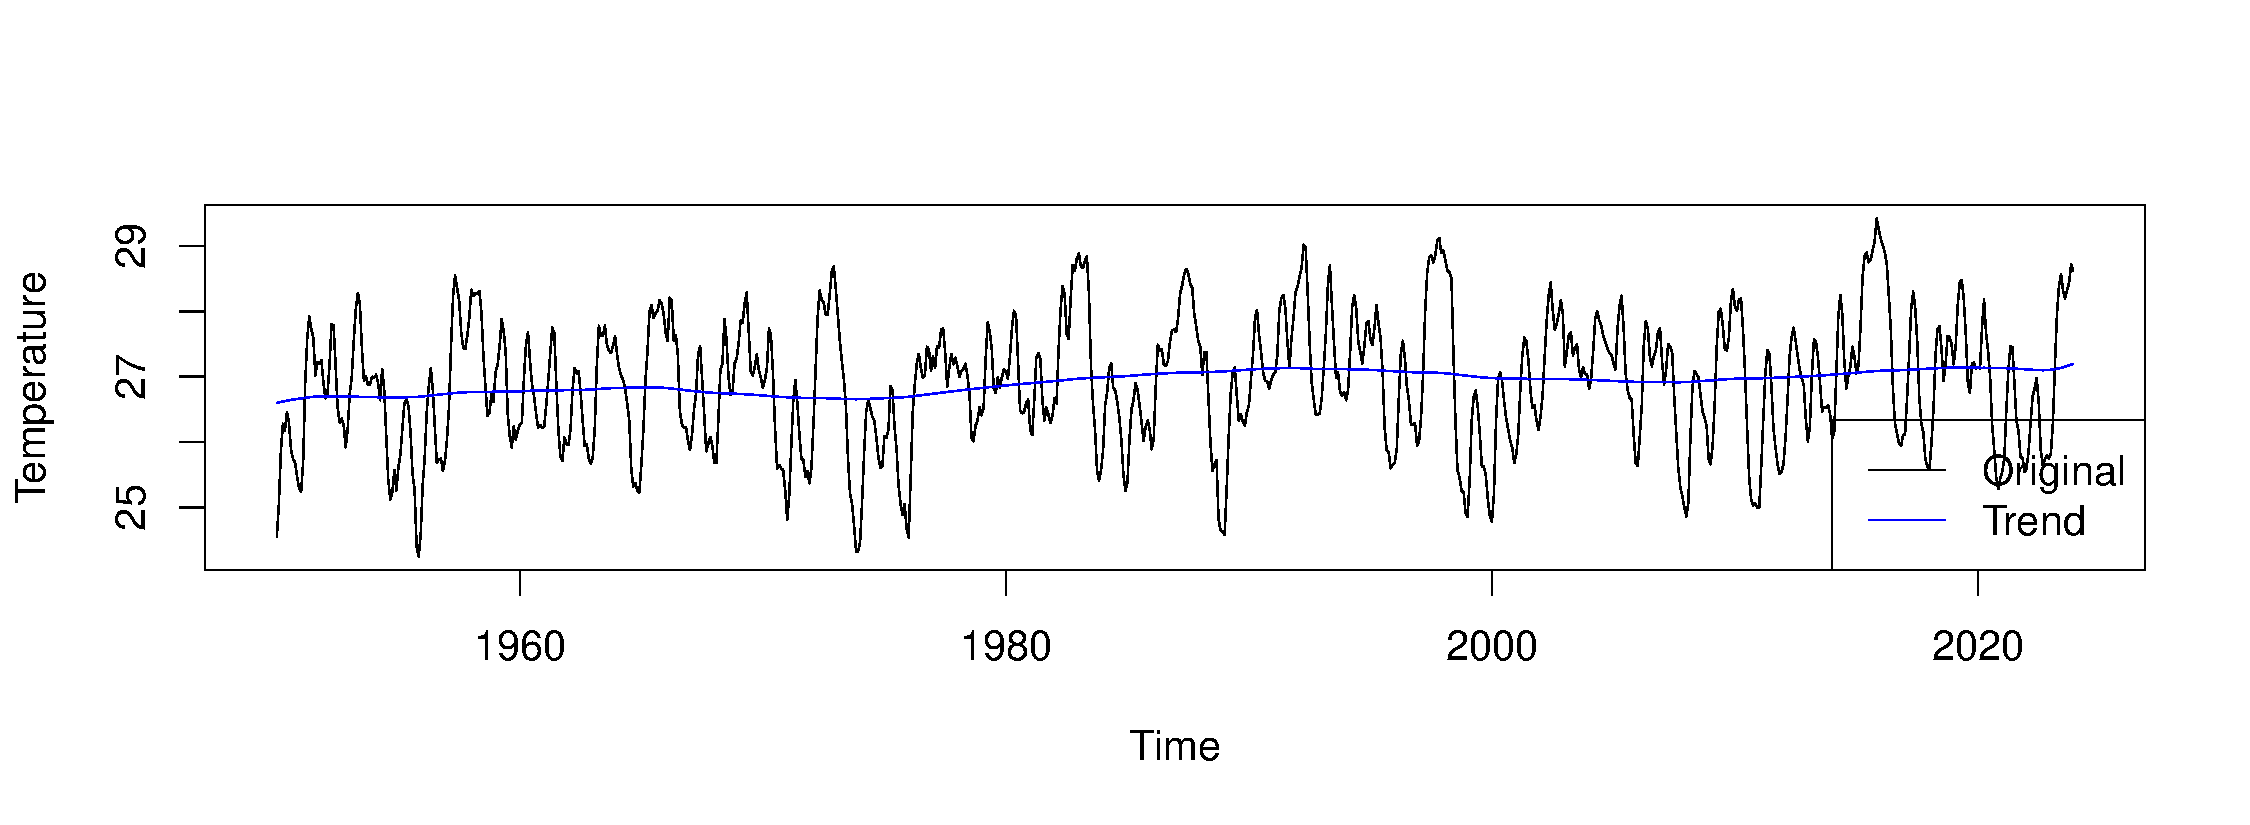
\includegraphics[width=\textwidth]{img/Nino_reconstruct_trend.pdf}\vspace{-2.8em}
    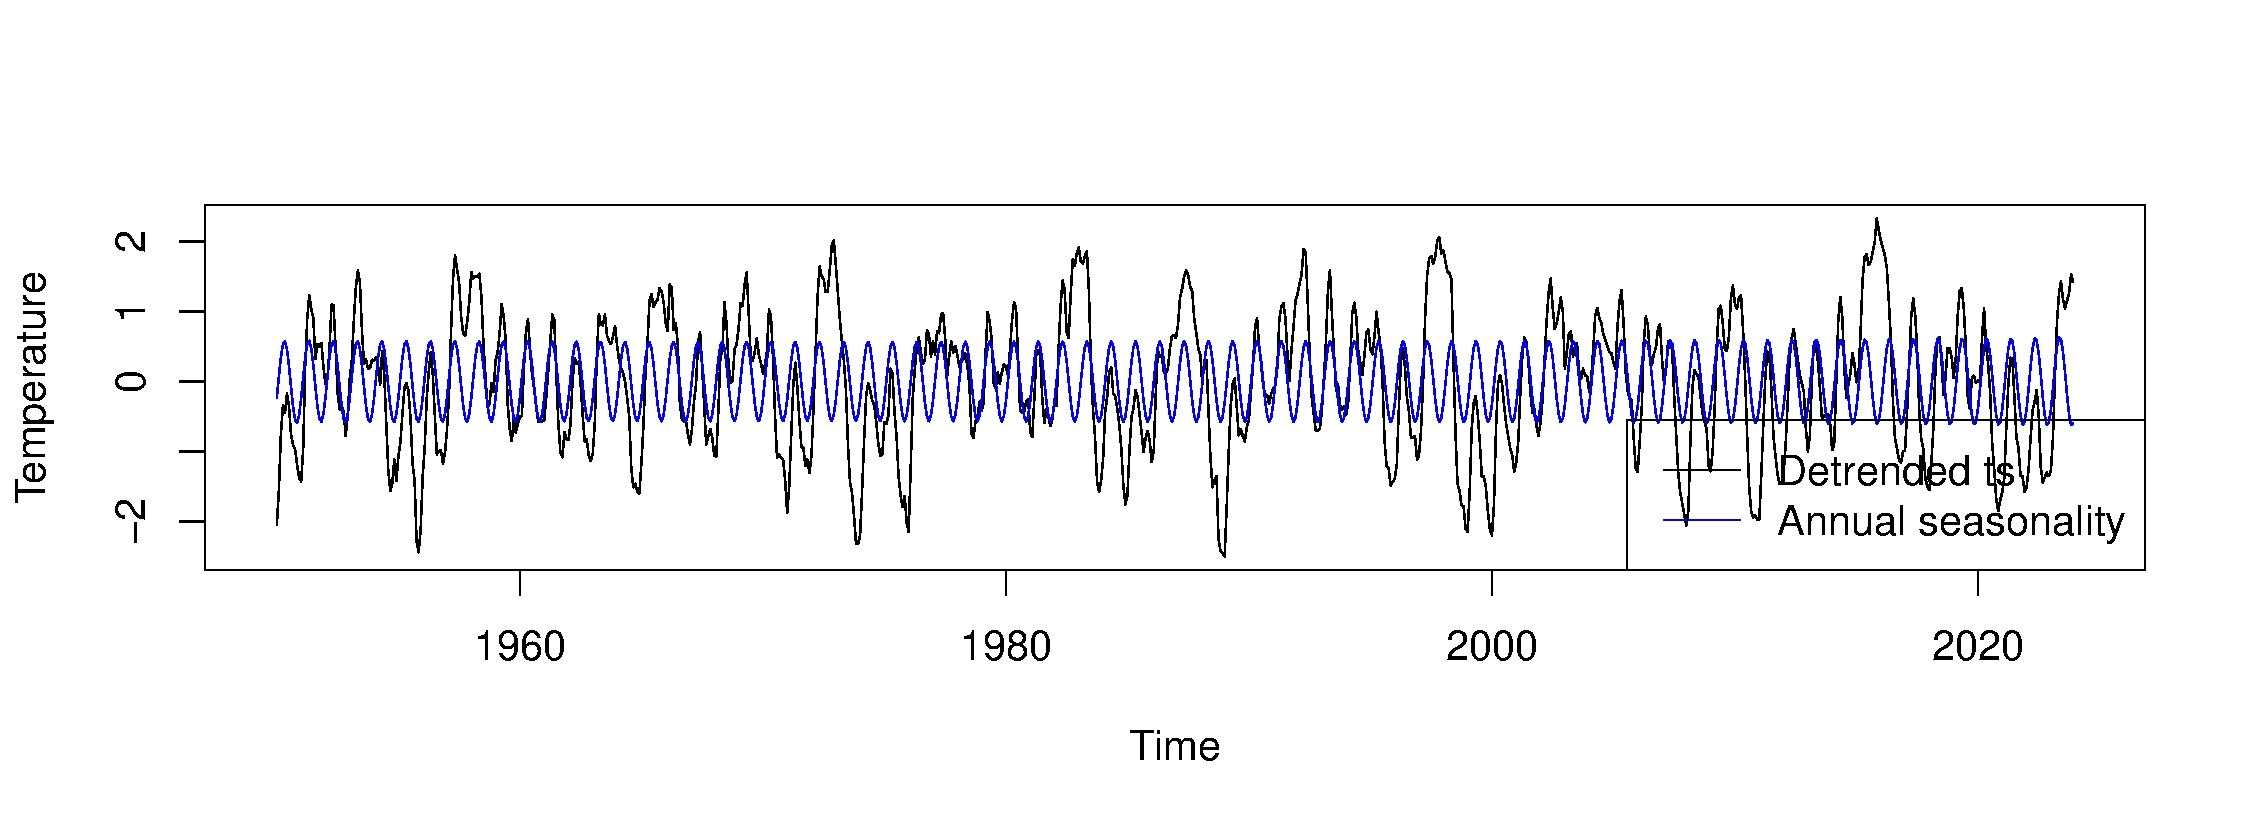
\includegraphics[width=\textwidth]{img/Nino_reconstruct_season.pdf}\vspace{-1em}
    Выделенный тренд ($L=120$) и годовая сезонность ($L=444$) (данные по месяцам)
  \end{figure}
\end{frame}

\begin{frame}{Анализ реального примера}
  \begin{figure}[h!]
    \centering
    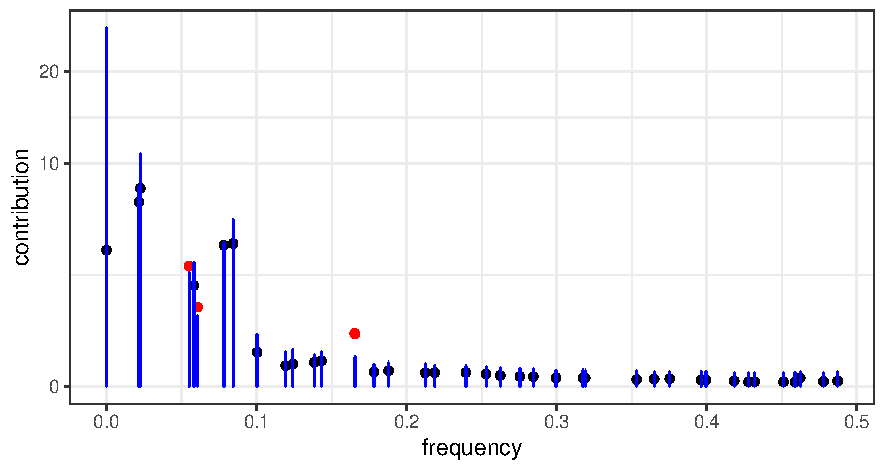
\includegraphics[width=0.8\textwidth]{img/Nino_mcssa.pdf}
    \caption{Результат работы MC-SSA ($\alpha=0.1$)}
    \label{Nino_mcssa}
  \end{figure}
  Значимыми являются четыре компоненты, две компоненты, имеющие \textbf{период} приблизительно $\mathbf{6}$, легко интерпретируются~---  это замеченная \textbf{полугодовая периодичность}.
\end{frame}

\section{}
\begin{frame}{Заключение}
  Мои результаты:
	\begin{enumerate}
		\item Был реализован метод Toeplitz MSSA в вариантах Block и Sum (на языке \textsf{R}) и на основе численных исследований рекомендуется использовать вариант Sum в виду численной эффективности и реализации, подходящей под пакет \textsf{Rssa}.
		\item Был выработан подход к сравнению критериев, построенных на основе радикальных, которые используют суррогатные выборки: выбирать наиболее мощный критерий среди не слишком радикальных.
		\item На основе этого подхода рекомендуется использовать модификацию Toeplitz Sum MC-MSSA.
    \item Проведены численные исследования по выбору оптимальной длины окна, степени искажения критерия при оценке параметров красного шума, а также случая мешающего сигнала. Однако эти проблемы оказались непростыми, поэтому требуется их дальнейшее исследование.
    \item Метод MC-SSA намного мощнее двух рассмотренных критериев в задаче обнаружения сигнала в красном шуме, особенно при малых частотах сигнала в альтернативе.
  \end{enumerate}
\end{frame}

\end{document}